% !TEX root = ../main.tex
%
\chapter{User Interface Design}
\label{sec:design}

The user interface was designed to be as simple as possible, while still providing all necessary functionality. 
The design of the prototype can be broken down into two main parts: a dashboard that gives an overview of all projects and a project section that provides users with the tools to create and edit NeRF models.

\section{Dashboard}

The dashboard is the first view that users see when opening the application. It shows all previously created projects and allows users to create new ones. 
Projects are represented as cards, showing the project name, a preview of on the provided input images (if present), and tags the indicate the current status of the project.
An additional card is present through which users can create a new project, by providing a name.
Projects can be opened by clicking a button on the respective card, when creating a new project, users are redirected to the project section.

\begin{figure}[htb]
  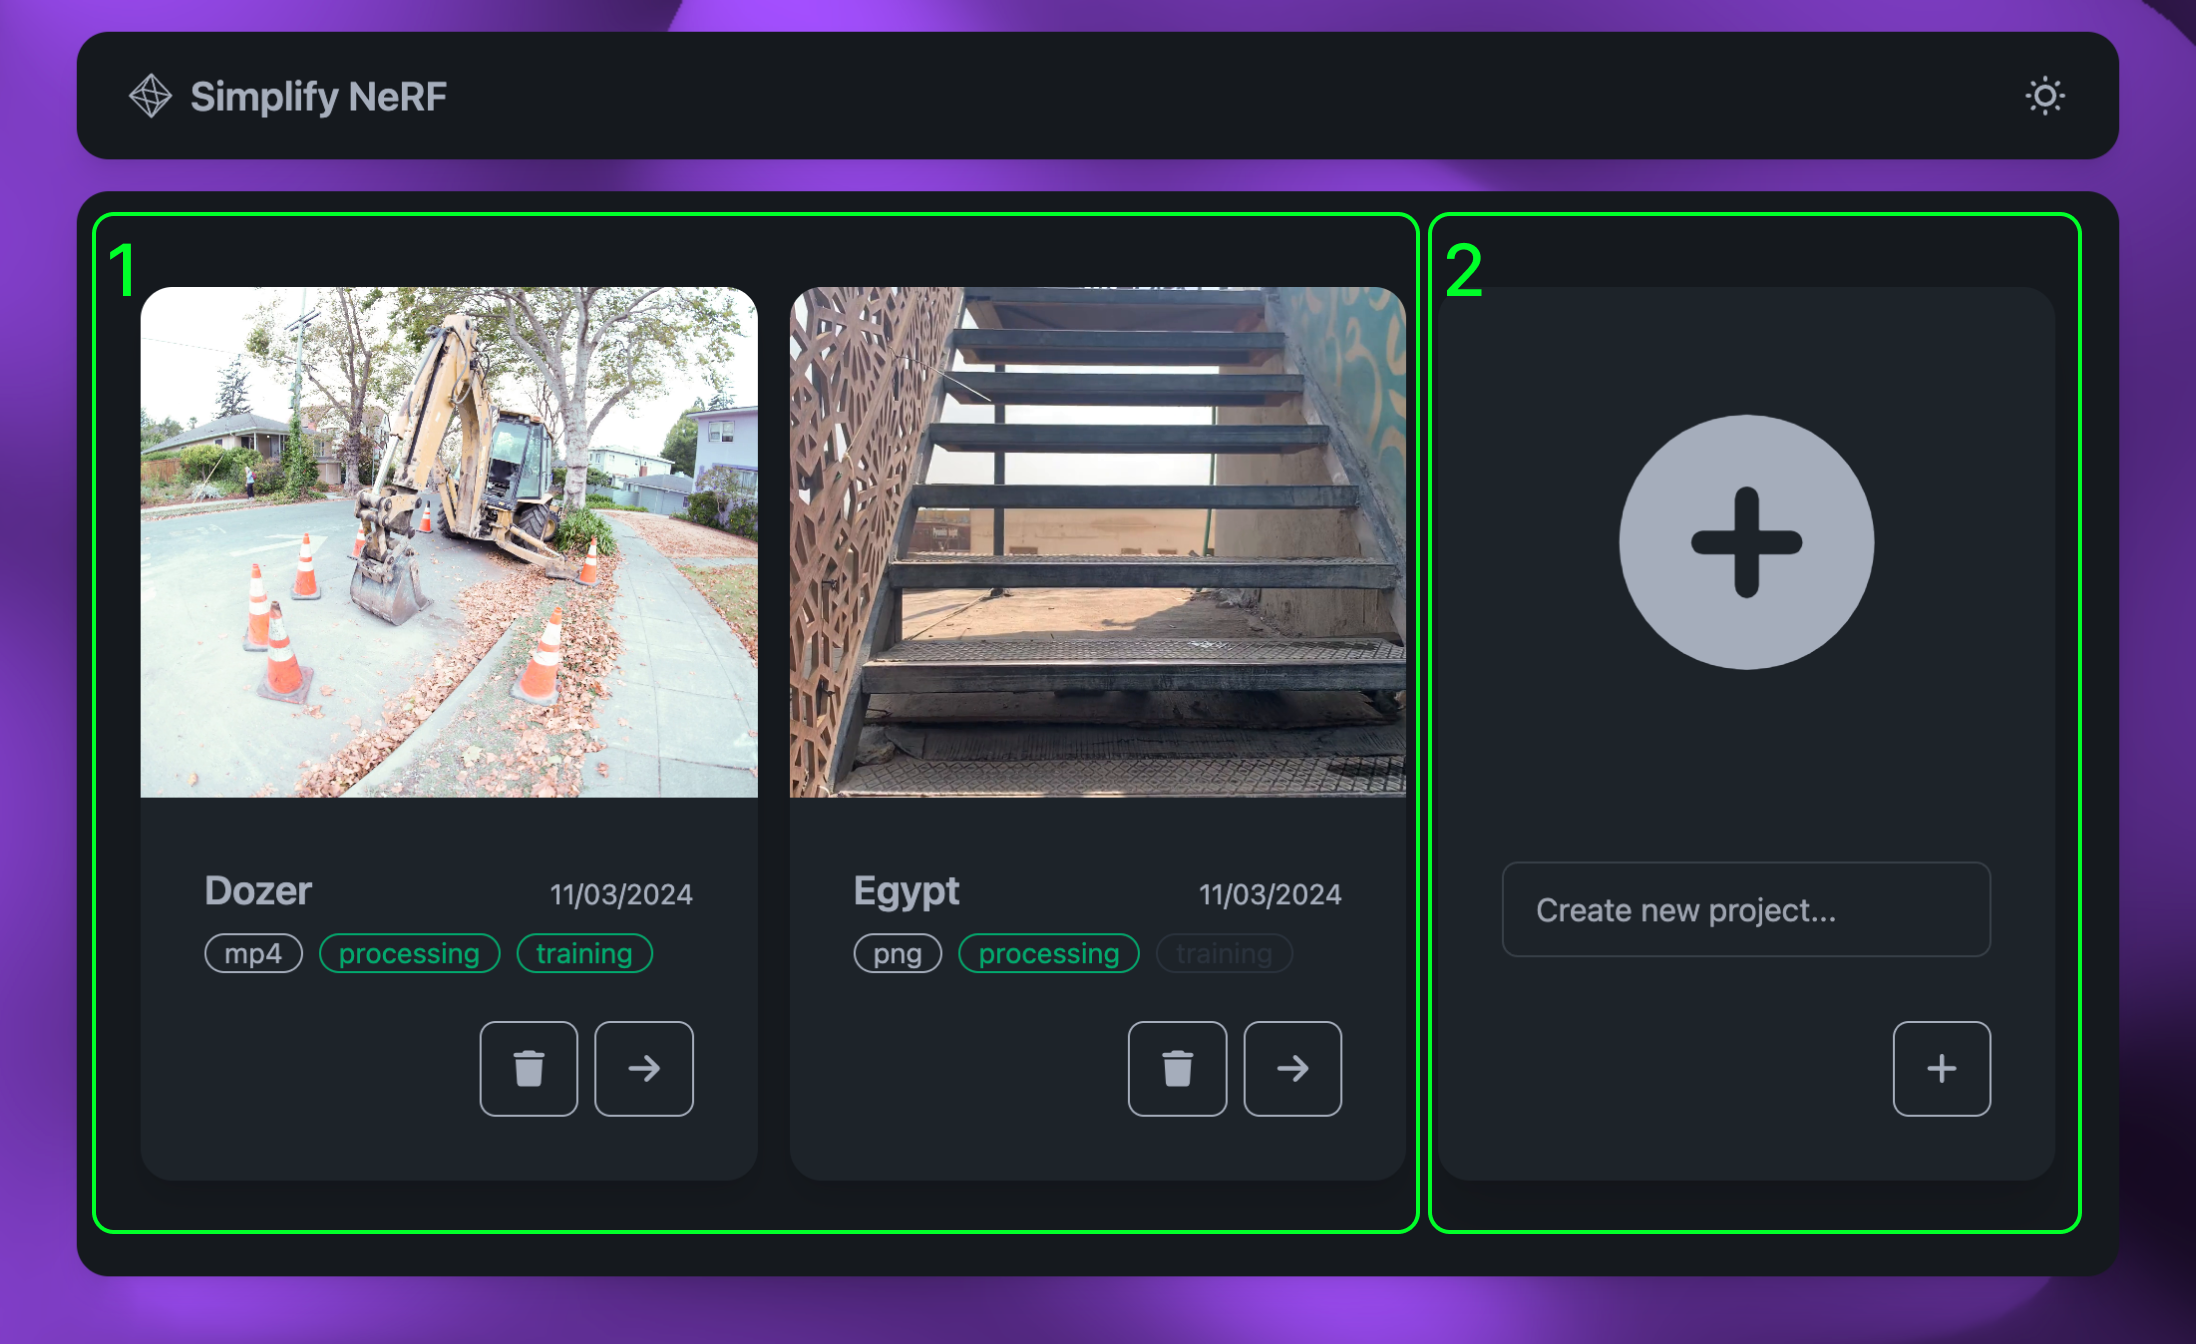
\includegraphics[width=\textwidth]{figures/view-overview.png}
  \caption{Dashboard}
  \label{fig:design:dashboard}
\end{figure}

\section{Project Section}

The project section is the core of the application, through which users can create and edit NeRF models.
The section is divided into three parts: the input section, the training section, and the rendering section.
Across all sections, users user can track there progress through a progress bar at the top of the screen, that also enables easy navigation between the different sections.

\subsection*{Input Section}

The input section combines the first few interactions, as mapped out in the user flow diagram.
First users are prompted to upload there input data, which can be done by dragging and dropping files into the browser window or by clicking a button to open a file dialog.
Files can be either a set of images or a video, and there are some guardrails in place to ensure that the input data is valid.
Once the input data is uploaded, it has to be processed before it can be used for training. 
The pre-processing can be configured by the user, this includes parameters such as the lense-type, or matching method.
Parameter input fields vary based on the type of input data, and are only shown when relevant.
Once the user is satisfied with the settings, they can start the pre-processing.
Feedback on the progress of the pre-processing is given through a console that shows the output of the process running on the server.
When the pre-processing is finished, the user can move on to the training section. 

\begin{figure}[htb]
  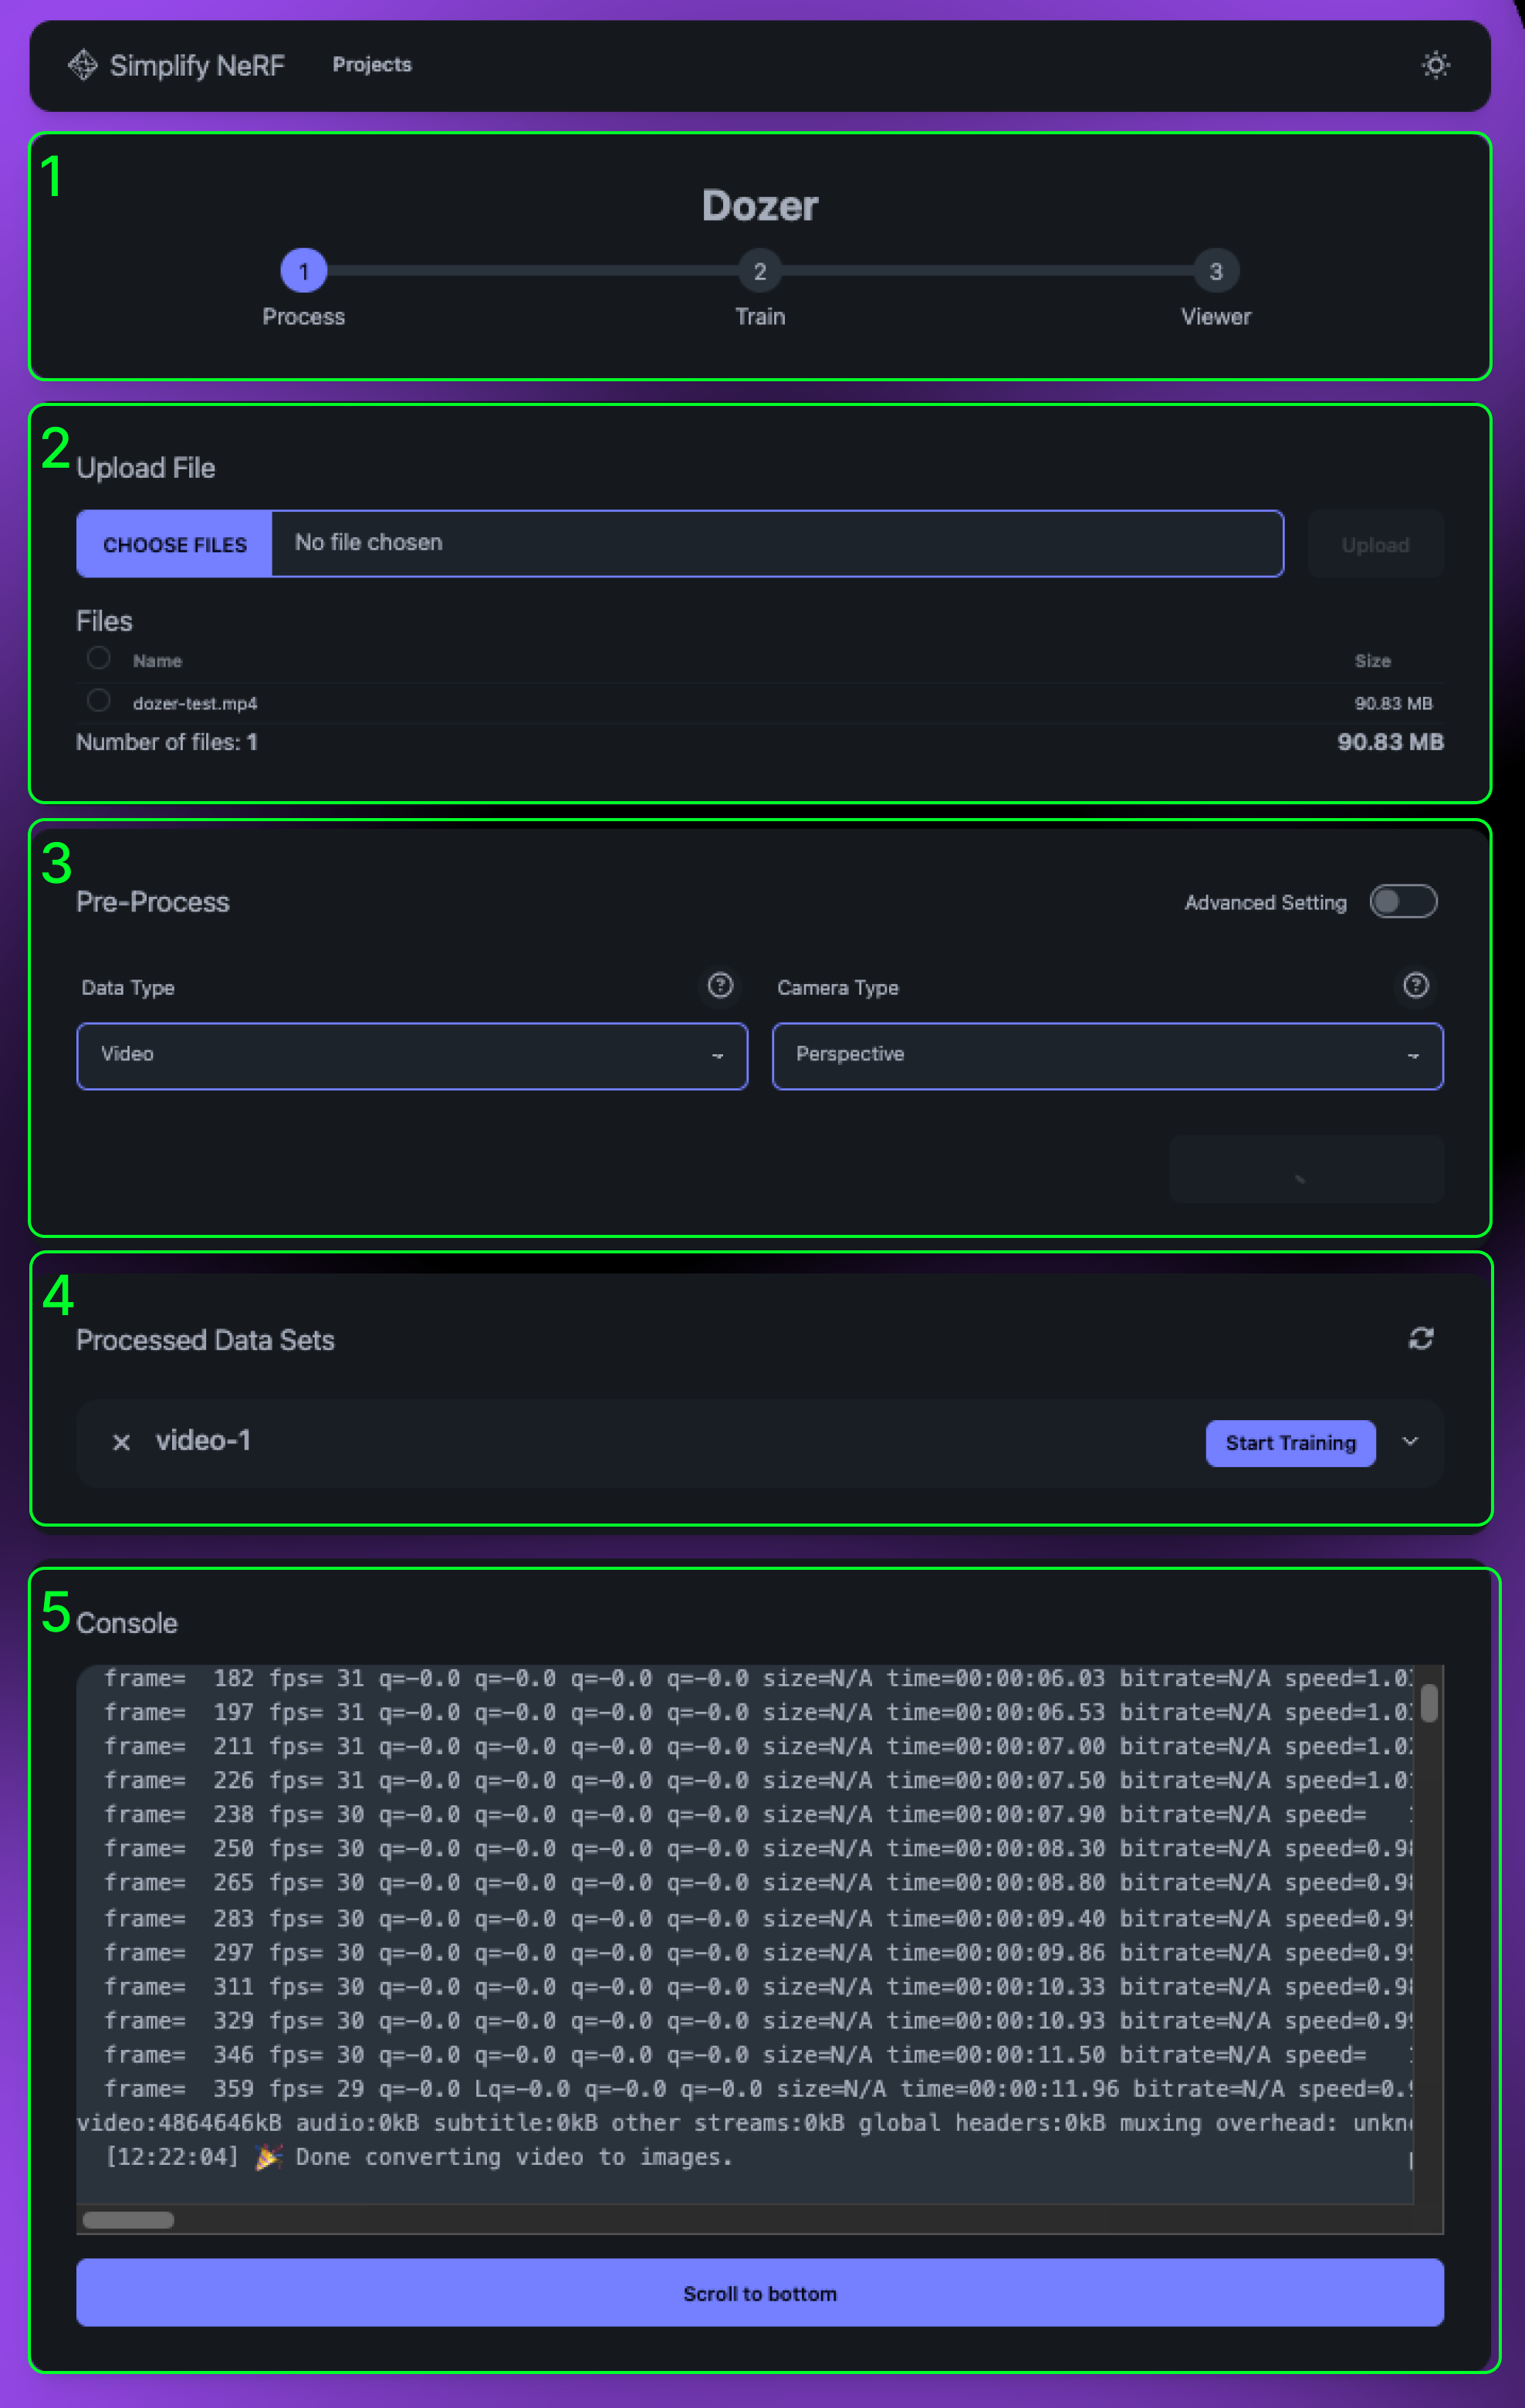
\includegraphics[width=\textwidth]{figures/view-process.png}
  \caption{Processing Input Data}
  \label{fig:design:input-section}
\end{figure}

In case the data was already pre-processed, a list ist visible that shows all available pre-processed data, and the user can select one to use for training.
Users can also inspect the configuration with which the data was pre-processed, and delete it if necessary.

\subsection*{Training Section}

The training section is structured similarly to the input section, with a form that allows users to configure the training process, and a console that shows the output of the training process running on the server.
When the user is satisfied with the configuration, they can start the training process.

\begin{figure}[htb]
  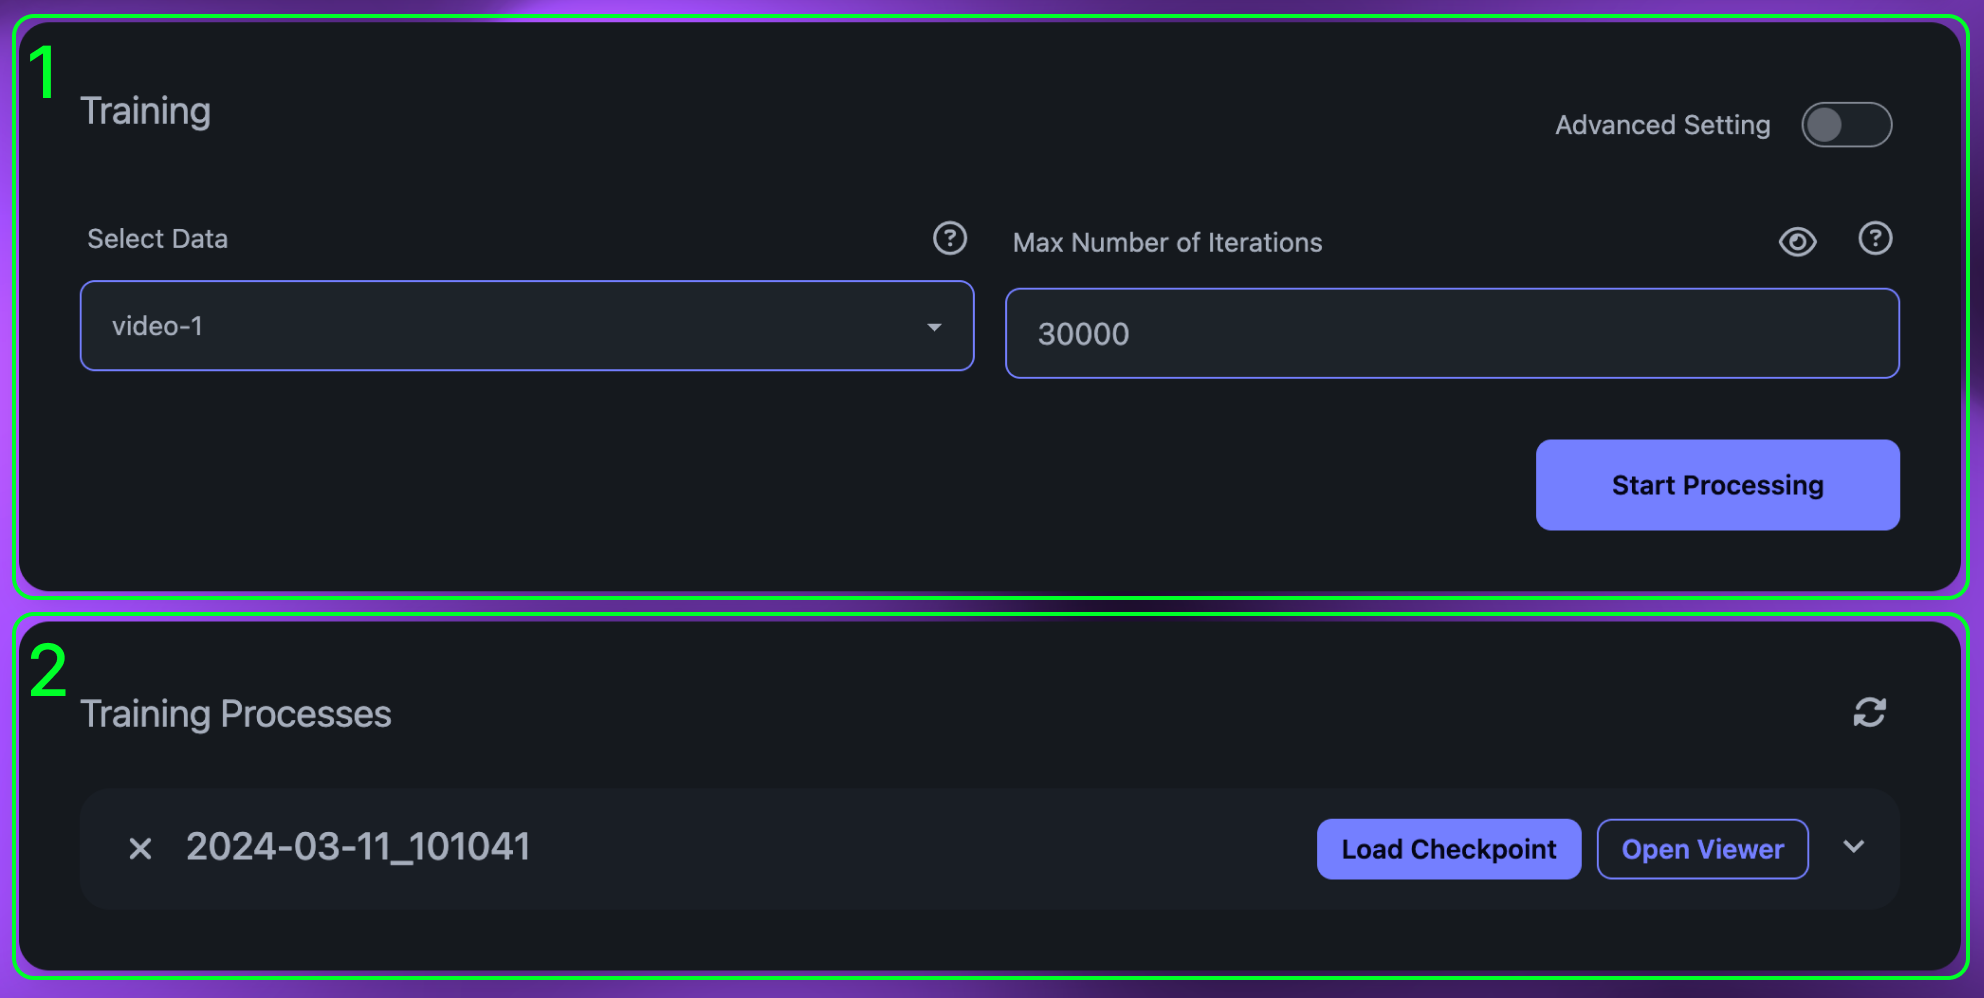
\includegraphics[width=\textwidth]{figures/view-train.png}
  \caption{Training Section}
  \label{fig:design:training-section}
\end{figure}


Previous training runs are listed, and users can inspect the configuration with which the training was run, and delete it if necessary. 
The viewer can be opened to inspect the results of the training run, or an existing checkpoint can be selected to continue training from that point.

\subsection*{Viewer Section}

The viewer section is the final step in the process, and allows users to inspect there NeRF model, while it is still training or after the training has finished.
At its core is the Nerfstudio Viewer that is integrated into the application. 
It provides users with all the functionality available in the standalone version, with a few integration that simplify the render process.
Instead of providing commands that have to be executed in the terminal, the rendering is started by clicking a button.

The renders are listed below the viewer, and once they finished processing, they can be downloaded to the users machine.

Due to the narrow layout of the page, the viewer can easily be opened in a new tab, to provide a better viewing experience.

\begin{figure}[htb]
  \includegraphics[width=\textwidth]{figures/view-viewer.png}
  \caption{Viewer Section}
  \label{fig:design:viewer-section}
\end{figure}

\section{Design Language}

\subsection*{Layout}

The layout of the application is kept minimalistic, its main objective is to guide the user through the process of creating a NeRF model, and keep them informed about the progress.

All elements of interest are group together, and placed into cards to provide a clear separation between different parts of the application.
Interactions that require previous user input, appear only when necessary, and are hidden by default.
As an example, in the processing section, only the upload card is visible, until the user has uploaded some data, then the processing card appears.
This helps user to focus on the task at hand, and guide them through the process.

\subsection*{Theming}

The application support a light and a dark theme, that can be toggled by the user and uses the user's system preference as a default.
The themes are designed to be easy on the eyes, and to provide a good contrast between different elements.
Interactive elements are highlighted with a purple color, to make them stand out.

The background of the application uses a gradient animation, that is subtle and does not distract from the content, but provides a more dynamic feel to the application.
